% Paper template for TAR 2022
% (C) 2014 Jan Šnajder, Goran Glavaš, Domagoj Alagić, Mladen Karan
% TakeLab, FER

\documentclass[10pt, a4paper, croatian]{article}

\usepackage{tar2023}

\usepackage[provide=*]{babel}

\usepackage[utf8]{inputenc}
\usepackage[pdftex]{graphicx}
\usepackage{booktabs}
\usepackage{amsmath}
\usepackage{amssymb}

\title{Nadopunjavanje slike korištenjem difuzijskih modela}

\name{Martin Bakač, Mislav Đomlija, Ivan Kapusta, Maksim Kos, Antonio Lukić, Jerko Šegvić}

\address{
University of Zagreb, Faculty of Electrical Engineering and Computing\\
Unska 3, 10000 Zagreb, Croatia\\ 
}
          
         
\abstract{
Cilj nadopunjavanja slike je nedostajuće piksele slike zamijeniti čim uvjerljivijim sadržajem. U projektu smo opisali i implementirali model za nadopunjavanje slika temeljen na difuziji. Trenirali smo difuzijski model na skupu podataka MNIST, impelemntirali RePaint \cite{repaint} petlju za popunjavanje slike te razvili sučelje za vizualizaciju maske, nepotpune slike i popunjene slike. Model uvjerljivo ispunjava slike.
}

\begin{document}

\maketitleabstract

\section{Nadopunjavanje slike}
Nadopunjavnje slike (engl. \emph{image inpainting}) je postupak u kojem nadopunjavamo segmente slike koji nedostaju. Nadopuna mora biti 
semantički smislena i u skladnom odnosu s poznatim dijelom slike. Zbog ovih čvrstih zahtjeva, modeli za nadopunjavanje slike moraju imati 
snažne generativne mogućnosti. Generativni difuzijski modeli, uz dobre generativne sposobnosti, omogućuju i manipulaciju latentnog prostora 
za ugradnju semantičke informacije. Popularni modeli za ovaj zadatak su još i generativne suparničke mreže 
(engl. \emph{generative adverserial networks}) i autoregresivni modeli. Problem takvih arhitketura je da moraju također naučiti i distribuciju
dijelova slike koji nedostaju. U praksi takvi modeli imaju problema sa neobičnim prazninama u slici ili sa prazninama s kojima se nisu
susreli prilikom treniranja


\section{Difuzijski modeli}
Difuzijski modeli su su klasa generativnih modela s latentnim varijablama \cite{diffusion}. Ideja difuzijskih modela je simulirati proces reverzne difuzije 
i naučiti model da iz poznate latentne distribucije konstruira elemente iz distribucije podataka. Svaki difuzijski model se sastoji od dva
osnovna elementa: unaprijedni proces i reverzni proces. Unaprijedni proces nema slobodne parametre, već se unaprijed definiranim 
transformacijama podatak postepeno pretvori u element latentne distribucije. Za distribuciju latentnog prostora odabrali smo normalnu razdiobu.
Dimenzija latentnog prostora jednaka je dimenziji prostora podatka. Unaprijedni proces može se promatrati kao markovljev lanac, i moguće je 
izvesti uvjetne distribuciju sljedećeg stanja na temelju trenutnog. Za distribuciju zadnjeg stanja lanca pretpostavljamo upravo latentnu 
distribuciju. Unatražnu distribuciju nije traktabilna te nju upravo procjenjujemo pomoću dubokog modela. 

\subsection{UNet}
Za predviđanje parametara difuzire $\mu_{n,\phi}$ i $\sigma^2_n$ koristili smo neuronsku mrežu arhitekture UNet.
UNet arhitektura se primijenjuje u području račulnalnog vida za semantičku segmentaciju i drugim domenama \cite{unet}.
Sastoji se od enkoderskog i dekoderskog dijela, s preskočnim vezama izmežu istih.
\begin{figure}
	\begin{center}
	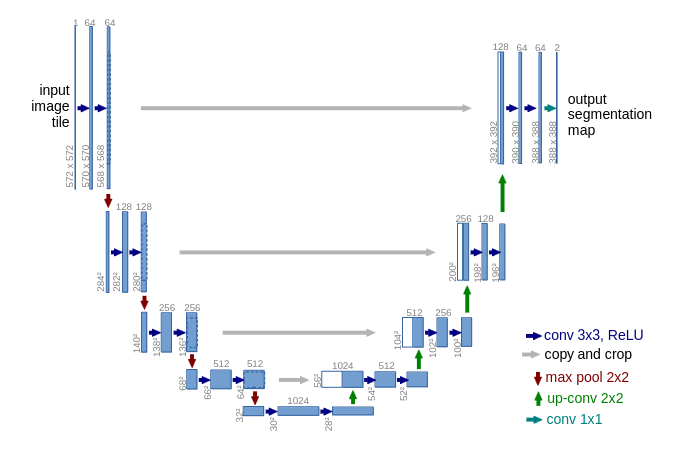
\includegraphics[width=\columnwidth]{images/unet.png}
	\caption{Arhitektura unet mreže. \cite{unet}}
	\label{fig:figure1}
	\end{center}
\end{figure}
U enkoderskom dijelu smanjujemo prostornu rezoluciju, a povećavamo broj kanala dok u dekoderskom dijelu radimo suprotno. 
Preskočne veze služe kako bi se očuvale prostorno relevanjtne informacije iz višil slojeva.
Kako bi očuvali informaciju u vremenski koracima difuzije $t$ koristimo vremenska ugrađivanja.
Jednostavanim višeslojnim perceptronom genereiramo naučeni vremenski-ovisan vektor koji se dodaje latentnoj prezentaciji.

\section{RePaint model}
RePaint je alogirtam za nadpounjavanje slike pomoću predtreniranog difuzijskog modela. Sam RePaint nema slobodne parametere te ga zato nije
potrebno učiti. To nam omogućava korištenje bilo kojeg difuzijskog modela \cite{repaint}. Također takav pristup nema pristranost prema nekim oblicima maski.
Algoritam funkcionira na sljedeći način. Vidljivi dio slike unaprijednim prolazom preslikamo u stanje $x_t \sim p_t$ . Nadopunjenu sliku 
generiramo iz latentnog prostora do stanja $x_t \sim q_t$. Sada na nadopunjenu sliku primjenimo inverznu masku i ove dvije slike zbrojimo. 
Njihov zbroj jednak je novom "latentnom prostoru" iz kojeg generiramo novu nadopunjenu sliku. Ova iteracija se ponavlja dok se cijeli reverzni
proces ne izvrši to jest do $t = 0$
\begin{figure}
	\begin{center}
	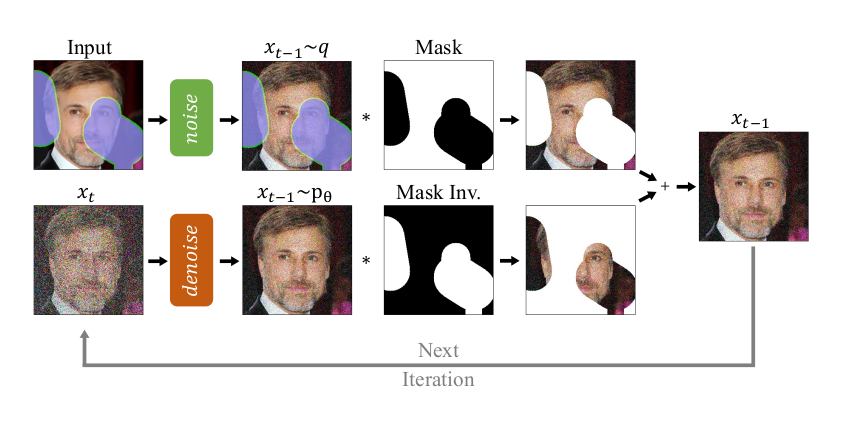
\includegraphics[width=\columnwidth]{images/repaint.png}
	\caption{Slikovni prikaz RePaint algoritma \cite{repaint}}
	\label{fig:figure2}
	\end{center}
\end{figure}

\section{Rezultati}
Kako bi testirali funkcionalnost našeg modela, maskirali smo nekoliko uzoraka iz skupa MNIST i predali modelu da ih dopuni (slika 2).
Model je uvjerljivo popunio maskirane djelove slika u većini slučajeva.
\begin{figure}
	\begin{center}
	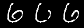
\includegraphics[width=\columnwidth]{../repaint_output/inpainted_combined_6.png}
	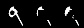
\includegraphics[width=\columnwidth]{../repaint_output/inpainted_combined_7.png}
	
\includegraphics[width=\columnwidth]{../repaint_output/inpainted_combined_8.png}
	\caption{Originalna slika, maskirana slika i rezultati nadopunjavanja}
	\label{fig:figure3}
	\end{center}
\end{figure}

\section{Zaključak}

U ovom radu istražili smo problem nadopunjavanja slike koristeći difuzijske modele. Difuzijski modeli pokazali su se kao obećavajuća klasa generativnih modela zbog svoje sposobnosti učenja latentnih reprezentacija kroz reverzni proces difuzije. Koristeći unaprijedni i reverzni proces, ovi modeli omogućuju postupno dodavanje i uklanjanje šuma na podacima, što omogućuje generiranje realističnih nadopuna slika.

Proveli smo implementaciju modela temeljenog na difuziji za nadopunjavanje slika i testirali ga na skupu podataka MNIST. Eksperimentalni rezultati pokazuju da difuzijski modeli mogu generirati vizualno uvjerljive nadopune čak i za slike s kompleksnim uzorcima nedostajućih područja. Prednosti ovakvog pristupa uključuju:

\begin{itemize}
    \item \textbf{Fleksibilnost maskiranja:} RePaint algoritam, korišten u ovom radu, ne pokazuje pristranost prema određenim oblicima maski, što ga čini generalno primjenjivim na različite vrste ulaznih podataka.
    \item \textbf{Korištenje postojećih modela:} Reverzni proces omogućuje iskorištavanje predtreniranih difuzijskih modela bez potrebe za dodatnim treniranjem, što značajno smanjuje računalne zahtjeve.
    \item \textbf{Robusnost:} Difuzijski modeli pokazali su robusnost prema nepoznatim obrascima praznina, za razliku od nekih tradicionalnih pristupa poput generativnih suparničkih mreža (GAN-ova).
\end{itemize}

Međutim, izazovi ostaju u smislu optimizacije performansi i brzine generiranja. Naši eksperimenti sugeriraju potrebu za daljnjim istraživanjem arhitektura difuzijskih modela kako bi se poboljšala kvaliteta nadopuna i smanjilo vrijeme izvođenja reverznih procesa.

Rezultati ovog rada doprinose razumijevanju primjene difuzijskih modela u nadopunjavanju slika i otvaraju mogućnosti za njihovu primjenu u širem spektru zadataka u domeni računalnog vida.


%\section*{Acknowledgements}

\bibliographystyle{tar2023}
\bibliography{report} 

\end{document}
